\documentclass[man, fleqn, noextraspace]{apa6}
\usepackage{lmodern}
\usepackage{amssymb,amsmath}
\usepackage{ifxetex,ifluatex}
\usepackage{fixltx2e} % provides \textsubscript
\ifnum 0\ifxetex 1\fi\ifluatex 1\fi=0 % if pdftex
  \usepackage[T1]{fontenc}
  \usepackage[utf8]{inputenc}
\else % if luatex or xelatex
  \ifxetex
    \usepackage{mathspec}
  \else
    \usepackage{fontspec}
  \fi
  \defaultfontfeatures{Ligatures=TeX,Scale=MatchLowercase}
\fi
% use upquote if available, for straight quotes in verbatim environments
\IfFileExists{upquote.sty}{\usepackage{upquote}}{}
% use microtype if available
\IfFileExists{microtype.sty}{%
\usepackage{microtype}
\UseMicrotypeSet[protrusion]{basicmath} % disable protrusion for tt fonts
}{}
\usepackage{hyperref}
\hypersetup{unicode=true,
            pdftitle={Data Visdualization on Madarin Vowels},
            pdfauthor={Teresa Chen, Jun Lang, Steffi Hung, \& Ting-fen Lin},
            pdfkeywords={Madarin, Vowels, Native speaker, Non-native speaker},
            pdfborder={0 0 0},
            breaklinks=true}
\urlstyle{same}  % don't use monospace font for urls
\usepackage{graphicx,grffile}
\makeatletter
\def\maxwidth{\ifdim\Gin@nat@width>\linewidth\linewidth\else\Gin@nat@width\fi}
\def\maxheight{\ifdim\Gin@nat@height>\textheight\textheight\else\Gin@nat@height\fi}
\makeatother
% Scale images if necessary, so that they will not overflow the page
% margins by default, and it is still possible to overwrite the defaults
% using explicit options in \includegraphics[width, height, ...]{}
\setkeys{Gin}{width=\maxwidth,height=\maxheight,keepaspectratio}
\IfFileExists{parskip.sty}{%
\usepackage{parskip}
}{% else
\setlength{\parindent}{0pt}
\setlength{\parskip}{6pt plus 2pt minus 1pt}
}
\setlength{\emergencystretch}{3em}  % prevent overfull lines
\providecommand{\tightlist}{%
  \setlength{\itemsep}{0pt}\setlength{\parskip}{0pt}}
\setcounter{secnumdepth}{0}
% Redefines (sub)paragraphs to behave more like sections
\ifx\paragraph\undefined\else
\let\oldparagraph\paragraph
\renewcommand{\paragraph}[1]{\oldparagraph{#1}\mbox{}}
\fi
\ifx\subparagraph\undefined\else
\let\oldsubparagraph\subparagraph
\renewcommand{\subparagraph}[1]{\oldsubparagraph{#1}\mbox{}}
\fi

%%% Use protect on footnotes to avoid problems with footnotes in titles
\let\rmarkdownfootnote\footnote%
\def\footnote{\protect\rmarkdownfootnote}


  \title{Data Visdualization on Madarin Vowels}
    \author{Teresa Chen\textsuperscript{3}, Jun Lang\textsuperscript{2}, Steffi
Hung\textsuperscript{2}, \& Ting-fen Lin\textsuperscript{1}}
    \date{}
  
\shorttitle{Final Project in EDLD 610: Introduction to Data Science with R}
\affiliation{
\vspace{0.5cm}
\textsuperscript{1} Department of Human Physiology\\\textsuperscript{2} Department of East Asian Languages \& Linguistics\\\textsuperscript{3} Communication Disorders \& Sciences}
\keywords{Madarin, Vowels, Native speaker, Non-native speaker}
\usepackage{csquotes}
\usepackage{upgreek}
\captionsetup{font=singlespacing,justification=justified}

\usepackage{longtable}
\usepackage{lscape}
\usepackage{multirow}
\usepackage{tabularx}
\usepackage[flushleft]{threeparttable}
\usepackage{threeparttablex}

\newenvironment{lltable}{\begin{landscape}\begin{center}\begin{ThreePartTable}}{\end{ThreePartTable}\end{center}\end{landscape}}

\makeatletter
\newcommand\LastLTentrywidth{1em}
\newlength\longtablewidth
\setlength{\longtablewidth}{1in}
\newcommand{\getlongtablewidth}{\begingroup \ifcsname LT@\roman{LT@tables}\endcsname \global\longtablewidth=0pt \renewcommand{\LT@entry}[2]{\global\advance\longtablewidth by ##2\relax\gdef\LastLTentrywidth{##2}}\@nameuse{LT@\roman{LT@tables}} \fi \endgroup}


\DeclareDelayedFloatFlavor{ThreePartTable}{table}
\DeclareDelayedFloatFlavor{lltable}{table}
\DeclareDelayedFloatFlavor*{longtable}{table}
\makeatletter
\renewcommand{\efloat@iwrite}[1]{\immediate\expandafter\protected@write\csname efloat@post#1\endcsname{}}
\makeatother

\authornote{Steffi and Jun are the owner of the dataset. They
have the correct permissions to make the dataset public.

Correspondence concerning this article should be addressed to Teresa
Chen, Rm.52 Gerlnger Annex, University of Oregon, OR 9740. E-mail:
\href{mailto:szuhuac@uoregon.edu}{\nolinkurl{szuhuac@uoregon.edu}}}

\abstract{

}

\begin{document}
\maketitle

{
\setcounter{tocdepth}{5}
\tableofcontents
}
\newpage

\section{Introduction}\label{introduction}

It is generally agreed that Mandarin Chinese has a five-vowel system
(see Hinton, Nichols, \& Ohala, 2006). These five vowels are {[}yi{]},
{[}yu{]}, {[}wu{]}, {[}en{]} and {[}ai{]}. Among these vowels, the mid
vowel has four allophones: {[}e{]}, {[}o{]}, {[}en{]} and {[}e{]}; and
the low vowel has two allophones: {[}ai{]} and {[}ao{]}. However, little
attention has been paid to the individual variances when producing these
nine vowels. Few researchers did empirical studies to examine Ashby and
Maidment (2005) vowel space of Chinese. In order to fill these gaps,
this study investigates the vowel distribution of native Chinese
speakers, aiming to determine whether native Chinese speakers show
similar patterns when producing Chinese vowels and whether their
patterns look similar to Roach's (2004) proposal of Chinese vowel chart.
In addition, this current work examines the vowel distribution of
American English learners of Chinese, with the purpose of finding out
whether non-native speakers perform similarly to native speakers in the
vowel production.

\begin{figure}
\centering
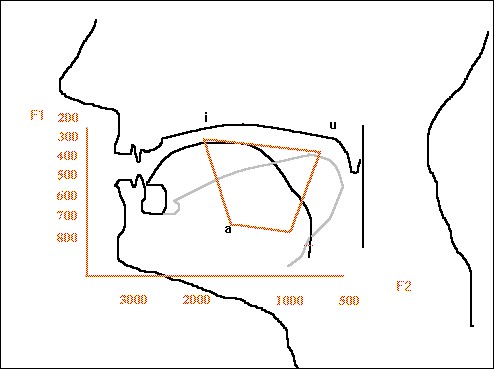
\includegraphics{picture/mouth.jpg}
\caption{vocal tract}
\end{figure}

\section{Methods}\label{methods}

\subsection{Participants}\label{participants}

Six female native (L1) Mandarin speakers and six female non-native (L2)
Mandarin speakers participated in the study. The mean age of the L1
Mandarin speakers was 26.3 (range: 23-30) and that of the L2 Mandarin
speakers was 22.3 (range: 18-28). Among L1 Mandarin speakers, two
speakers were from northern Mainland China (Beijing and Tianjin), three
speakers were from southern Mainland China (Nanjing, Chengdu and
Chongqing), and one speaker was from Taiwan. The Taiwanese participant
identified Mandarin as her most fluent language. All the six L2 Mandarin
speakers' native language was American English. They were all novice-low
learners who enrolled in first-year accelerated Chinese language course
at the same university. They had learned Mandarin for six months and
none of them had any study-abroad experience.

\subsection{Speech materials}\label{speech-materials}

We prepared nine Chinese sentences for speech materials. Each sentence
includes one of the following nine vowels: {[}yi{]}, {[}yu{]}, {[}wu{]},
{[}e{]}, {[}o{]}, {[}en{]}, {[}e{]}, {[}ai{]}, {[}ao{]}. Each vowel
appears after the aspirated bilabial stop {[}p{]} with a high tone (55).

\subsection{Procedure}\label{procedure}

Productions were elicited in a sentence-repetition oral task. Non-native
speakers (NNS) and native Chinese speakers (NS) were asked to read the
sentences twice. All participants read the speech materials for practice
once before recording. Recordings were made in a quiet study room in the
library using Praat Sound Recorder with 44,100 Hz sampling frequency,
and then these recordings were saved as wav files on a laptop. Formant 1
(F1) and Formant 2 (F2) were measured in the vowel mid-point for each
vowel shown in the spectrogram. All measurement was conducted using
Praat program on the same laptop. After the measurement, the mean F1 and
F2 values were plotted in charts using the program R to generate vowel
distribution for each speaker.

\section{Results and discussion}\label{results-and-discussion}

\subsection{Native speaker patterns}\label{native-speaker-patterns}

Table 1 shows the mean F1 and F2 values of nine Chinese vowels for
native speakers. Regarding F2 values, data shows that {[}yi{]} had the
highest F2 values for all native speakers, and {[}wu{]} had the lowest
F2 values for NS2 and NS3, but not for NS1. As for F1 values, three NS
also had different lowest and highest values. While {[}yi{]} had the
lowest F1 value and {[}ao{]} had the highest F1 value for NS1 and NS3,
NS2's {[}yu{]} had the lowest F1 value and her {[}ai{]} had the highest
F1 value.

\begin{table}

\caption{\label{tab:table1}Formant by volwels among non-native and native groups}
\centering
\begin{tabular}[t]{llrrrr}
\toprule
group & vowel & F1\_mean & F2\_mean & F1\_sd & F2\_sd\\
\midrule
NNS & ai & 913.33 & 1513.83 & 47.14 & 161.28\\
NNS & ao & 901.50 & 1377.00 & 63.86 & 107.69\\
NNS & e & 640.33 & 1702.33 & 70.43 & 238.62\\
NNS & en & 651.33 & 1980.00 & 88.59 & 166.70\\
NNS & wo & 551.50 & 1043.67 & 49.79 & 61.90\\
\addlinespace
NNS & wu & 416.00 & 1122.83 & 69.62 & 196.96\\
NNS & ye & 520.67 & 2320.00 & 65.50 & 95.07\\
NNS & yi & 335.67 & 2646.50 & 46.03 & 100.61\\
NNS & yu & 321.50 & 1806.83 & 31.25 & 186.00\\
NS & ai & 910.33 & 1655.50 & 115.38 & 142.20\\
\addlinespace
NS & ao & 848.00 & 1305.17 & 59.50 & 147.96\\
NS & e & 596.83 & 1289.67 & 105.92 & 152.62\\
NS & en & 717.67 & 1850.50 & 40.10 & 101.96\\
NS & wo & 554.50 & 908.67 & 48.53 & 76.63\\
NS & wu & 335.00 & 840.00 & 15.63 & 56.02\\
\addlinespace
NS & ye & 556.83 & 2486.50 & 38.02 & 128.39\\
NS & yi & 308.33 & 2916.17 & 30.23 & 73.78\\
NS & yu & 309.17 & 2420.83 & 15.17 & 237.25\\
\bottomrule
\end{tabular}
\end{table}

Clearer vowel distribution for each native speaker can be seen in the
formant plots (Figure 1-3). According to the \enquote{vowel dispersion
principle}, the vowel quadrilateral can be viewed as \enquote{a
perceptual space in which vowels are located in the oral cavity} (Ashby
and Maidment, 2005). In this study, the vowel quadrilateral is shown as
formant plots where the Y-axis is F1 (Hz) that corresponds to the height
of the tongue position; while the X-axis is F2 (Hz) that indicates the
backness of the tongue position for each vowel (Figure 1 -3).

\begin{figure}
\centering
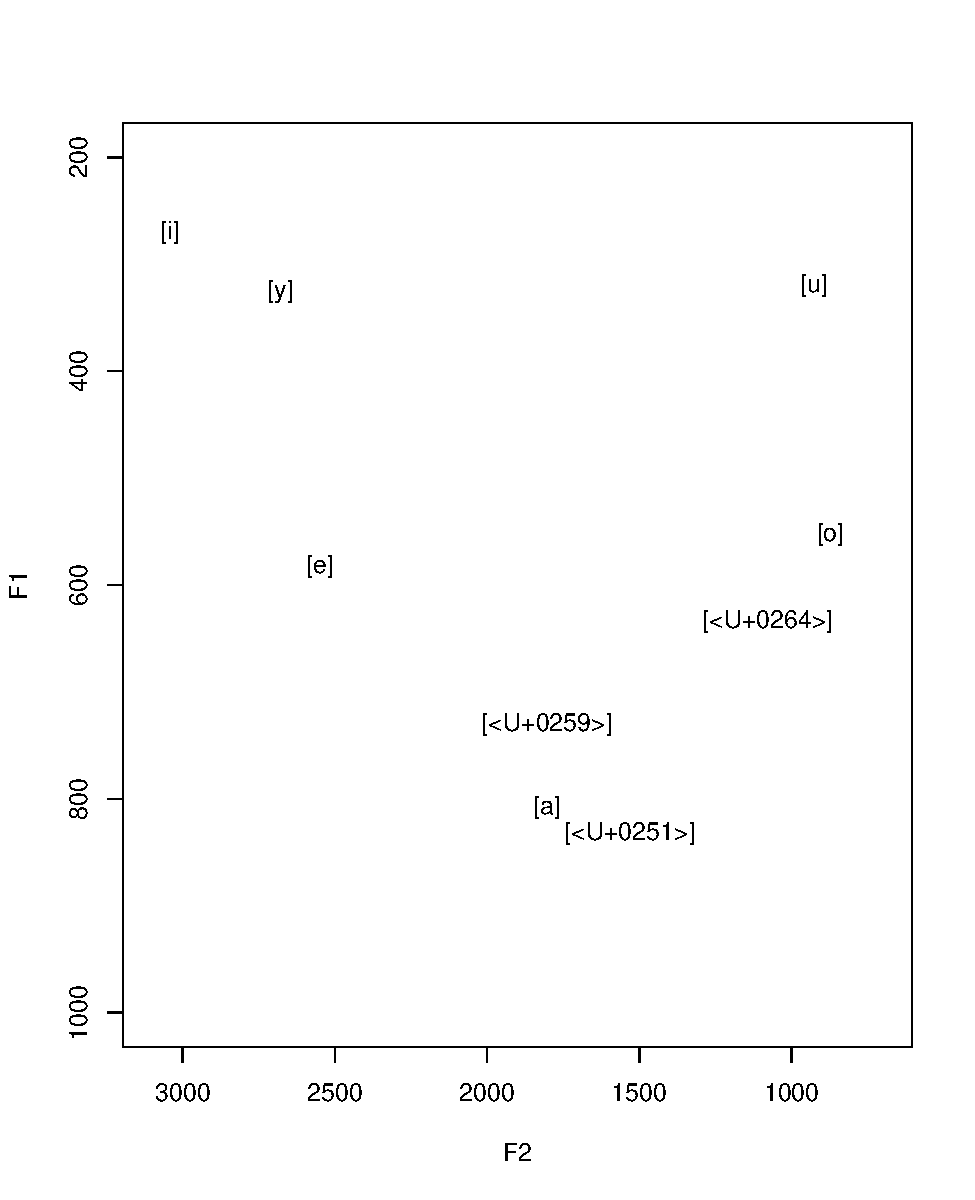
\includegraphics{Vowel_v2_files/figure-latex/figure1-1.pdf}
\caption{}
\end{figure}

\begin{figure}
\centering
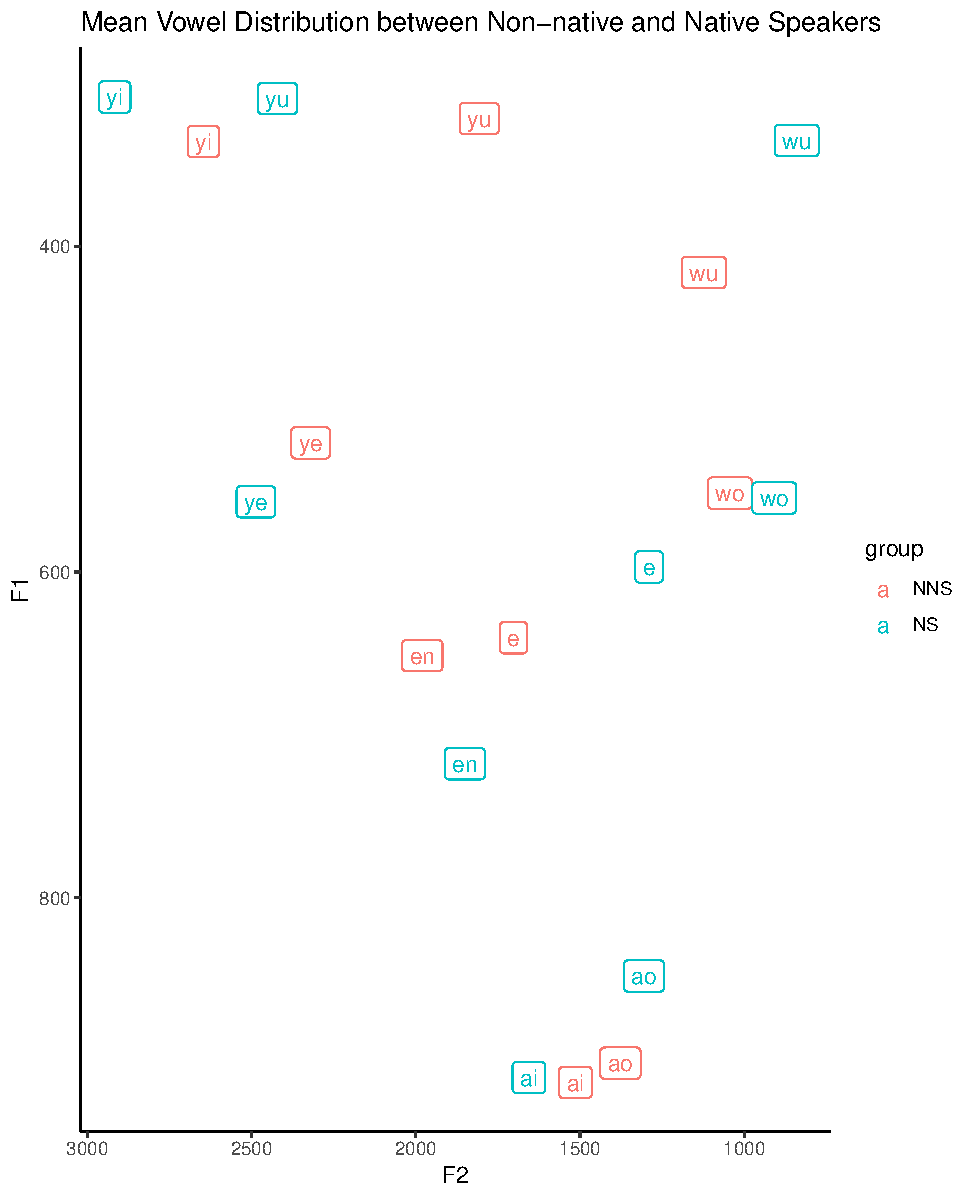
\includegraphics{Vowel_v2_files/figure-latex/figure2-1.pdf}
\caption{}
\end{figure}

\begin{figure}
\centering
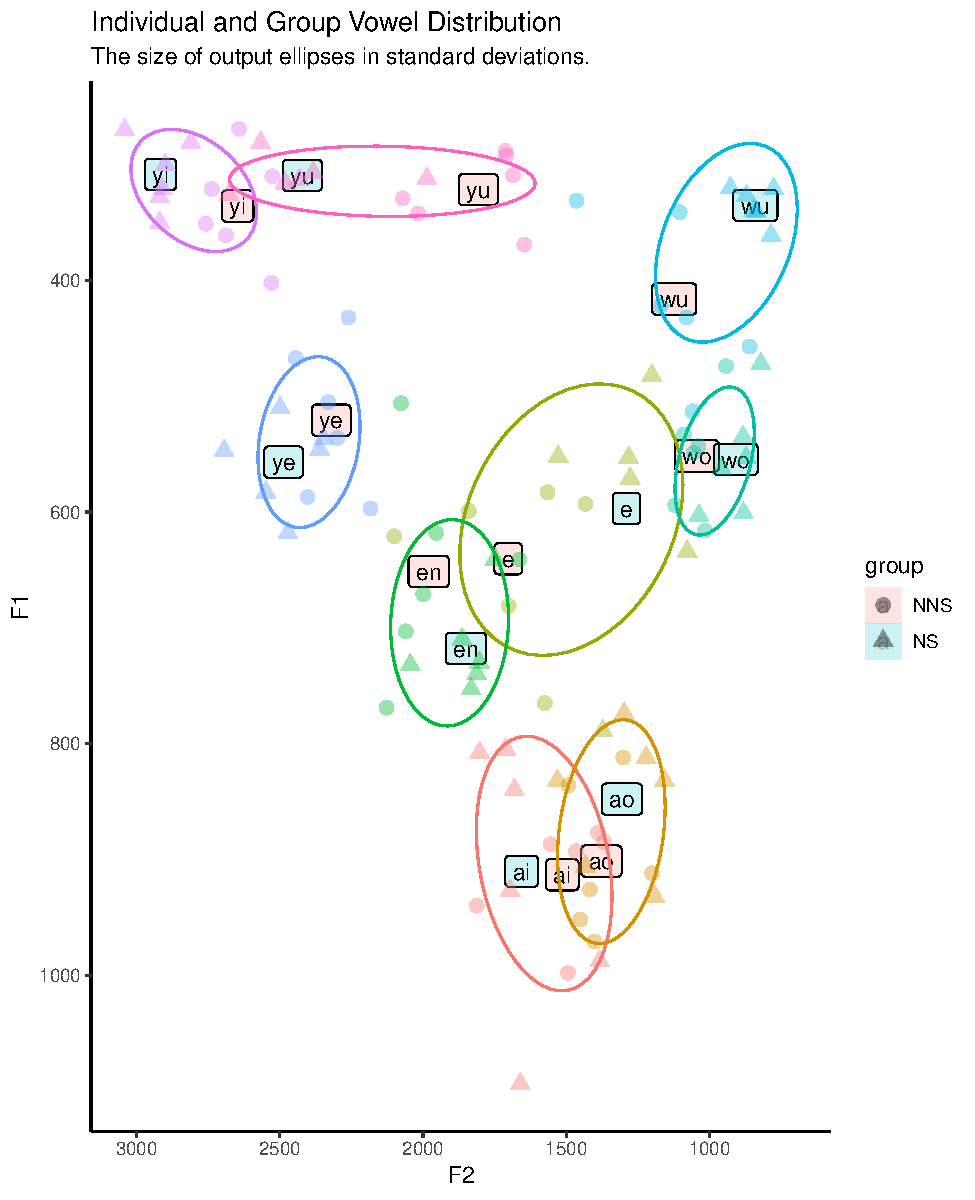
\includegraphics{Vowel_v2_files/figure-latex/figure3-1.pdf}
\caption{}
\end{figure}

\subsection{Second language
examination}\label{second-language-examination}

\section{Conclusion}\label{conclusion}

\newpage

\section{References}\label{references}

\begingroup
\setlength{\parindent}{-0.5in} \setlength{\leftskip}{0.5in}

\hypertarget{refs}{}
\hypertarget{ref-ashby2005}{}
Ashby, M., \& Maidment, J. (2005). \emph{Introducing phonetic science}.
Cambridge University Press.

\hypertarget{ref-hinton2006}{}
Hinton, L., Nichols, J., \& Ohala, J. J. (2006). \emph{Sound symbolism}.
Cambridge University Press.

\hypertarget{ref-roach2004}{}
Roach, P. (2004). British english: Received pronunciation. \emph{Journal
of the International Phonetic Association}, \emph{34}(2), 239--245.

\endgroup


\end{document}
